%\subsection{En Recursive Descent parser}
\begin{frame}
  \frametitle{En Recursive Descent parser}

  \begin{itemize}
    \item Håndskrevet parser vs. genereret parser
      \begin{itemize}
	\item Automatisk generering
	\item Tidskrævende
	\item Pålidelighed
	\item Skræddersy parseren
	\item Bedre forståelse for opbygning af parsere
	\item ''Black box''
      \end{itemize}
    \item Analyse af specifik syntaks
    \item Recursive descent, LL(1)-parser
    \item To klasser: Parser og AstNode
      \begin{itemize}
	\item Diverse metodekald $\rightarrow$ et abstrakt syntakstræ
	\item (\textbf{Type} type, \textbf{String} value, \textbf{int} line,
	  \textbf{int} offset)
      \end{itemize}
  \end{itemize}

\end{frame}

\begin{frame}
  \frametitle{En Recursive Descent parser}

  \begin{figure}
    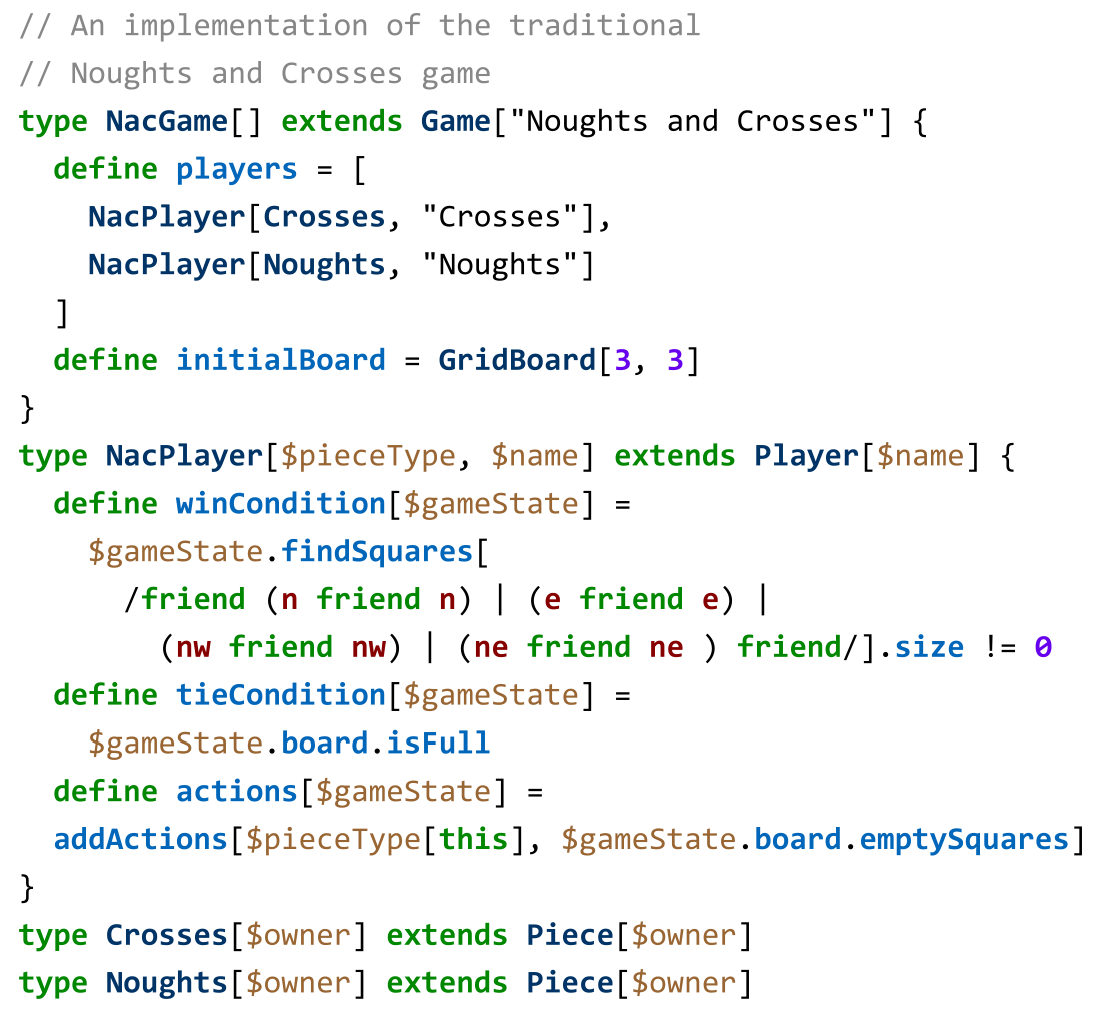
\includegraphics[width=0.6\linewidth]{billeder/krydsogbolle}
  \end{figure}

\end{frame}
